\chapter{Contributions and Research Plan}
\label{cha:plan}
\section{Contributions}
%Motivation
To explore how brain may recognise objects in its general, accurate, invariant and energy-efficient manner, this work proposes the use of a neuromorphic hardware system which includes a DVS retina connected to SpiNNaker, a real-time SNN simulator.
%Problem
Building a hand gesture recognition system based on this bespoke hardware for dynamic hand postures is a first step in the study of the ventral visual pathway in the brain.
%Methods
Inspired by the structures of the primary visual cortex, convolutional neural networks are modelled, and the V1-like neurons are simulated with both linear perceptrons and LIF neurons.
This model is position invariant to recognise five hand postures.

%Results
%The larger network of 74,210 neurons and 15,216,512 synapses runs smoothly in real-time on SpiNNaker using 290 cores within a 48-node board.
%The smaller network using 1/10 of the resources is able to recognise the postures in real-time with an accuracy about 86.4\% in average, which is 
%only 6.6\% lower than the former but with a better cost/performance ratio.

The detailed contributions are listed below:
\begin{itemize}
	\item Modelling a convolutional neural network which can recognise moving postures (position invariant) with V1-like neurons.
	\item Translation of conventional artificial neural networks of perceptrons to spiking neural networks of LIF neurons using the Siegert function.
	\item Configuring the SpiNNaker neuromorphic platform to communicate with the silicon retina to perform real-time posture recognition using spiking neurons.
	\item Maintaining software to make SpiNNaker receive correct recorded spikes and compare performance with perceptrons and also visualise the live neural activity in real time.
\end{itemize}
	
%In this paper, we implement a dynamic hand posture recognition system running completely on a hardware neuromorphic platform.
%The SNN based classifier is able to recognise moving hand postures instead of static digit or face recognition proposed before.
%The network model is translated from linear perceptrons to LIF spiking neurons with a 10\% drop of accuracy in 30~ms windowing;
%while the performance reaches and even exceeds the perceptrons version when the window length is set to 300~ms.
%Various network sizes are configured to explore the cost and performance trade-off.
%In the tests of linear perceptrons the recognition rate of the smaller network is \% lower for the template matching model and \% lower for the trained MLP model.
%For the SNN based real-time experiments, both the larger network with $74,320$ LIF neurons and $15,216,512$ synapses, and the smaller network with 1/10 of the neurons and 1/50 of the synapses run smoothly on SpiNNaker.
%The gap of recognition rate narrows when the spiking rate is sampled into wider frame of 300~ms.
%The recognition rates of both linear perceptrons (\%) and spiking neurons (\%) with 32 $\times$ 32 input resolution are adequate for the recognition of the moving hand postures.
%This work is a good attempt to start exploring the visual process of the brain.

%Later, we will look more into the overall network latency, which could be due to the system latency and the performance of the rate coding. 
\section{Achievements }
\subsection{Pulications}
\begin{itemize}

	\item Q. Liu and S. Furber, ``Real-time recognition of dynamic hand posture on a neuromorphic system." Artificial Neural Networks ICANN 2015. Springer Berlin Heidelberg. (Under review)


	\item Q. Liu, X. Lagorce, E. Stromatias, D. Emmanouilidou, R. Benosman, S. Furber and S. Liu, ``A large-scale, real-time sound localization on a neuromorphic platform." Neuromorphic Engineering. (Under proof reading of co-authors)

	\item Q. Liu, C. Patterson, S. Furber, Z. Huang, Y. Hou, and H. Zhang, ``Modeling populations of spiking neurons for fine timing sound localization." in Neural Networks (IJCNN), The 2013 International Joint Conference on, pp.1-8, Aug 2013.
\end{itemize}
\subsection{Workshops}
\begin{itemize}
	\item The 2014 CapoCaccia Cognitive Neuromorphic Engineering Workshop,\\ 28/04/2014 - 10/05/2014, Alghero, Sardinia, Italy 
	\item From Maps to Circuits: Models and Mechanisms for Generating Neural Connections, 28/07/2014 - 29/07/2014, Edinburgh UK
\end{itemize}
\section{Future Work} 
\begin{figure}[h!]
	\centering
	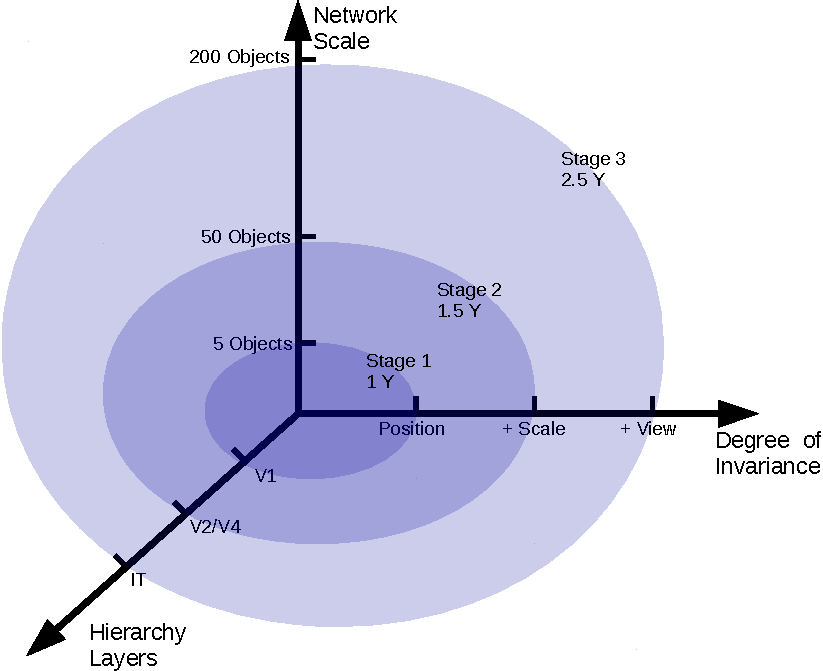
\includegraphics[width=0.75\textwidth]{pics/stages.pdf}
	\caption{3D representation of the research plan on the transformation-invariant object recognition system.
	Three milestones are pointed out indicating the expected targets of the object recognition networks.
	}
	\label{Fig:3Dplan}
\end{figure}
The proposed research plan is illustrated in Figure~\ref{Fig:3Dplan}, where the scope of the research is estimated in three dimensions.
To build a biologically-plausible object recognition system using spiking neurons, this work will be completed in three stages:
\begin{enumerate}
	\item Year 1, building a position-invariant object recognition system exploiting V1-like neurons to classify five hand postures. 
	\item Year 1.5, combining scale- with position-invariance on the object recognition system, and building the hierarchy ventral pathway to the V2/V4 layer to recognise 50 simple combined features such as gratings and contours.
	\item Year 2.5. integrating position-, scale- and view-invariance by modelling the hierarchical visual pathway up to the IT cortex and equipping the system with the ability to recognise 200 objects in real time.
\end{enumerate}
%The recognition ability of the system is measured in three dimensions: the hierarchy layers, degree of invariance and the network size.
 
This work will contribute to the understanding of biological visual processing by means of mimicking the neural activities in the ventral stream.
More importantly, the research will apply the accurate, rapid and robust approaches to artificial systems by exploring the brain's invariant object recognition.
The performance of the real-time recognition system will be tested on each milestone to validate the success of the models.
The neural activities and recognition rate will also be compared with biological data.

The key research steps are listed in Figure~\ref{Fig:gantt}.
Since the incremental work flow is hard to present in Gantt charts, only the work for the first milestone is shown.
The subsequent sections will outline the key research stages.



\begin{figure}[h!]
	\centering
	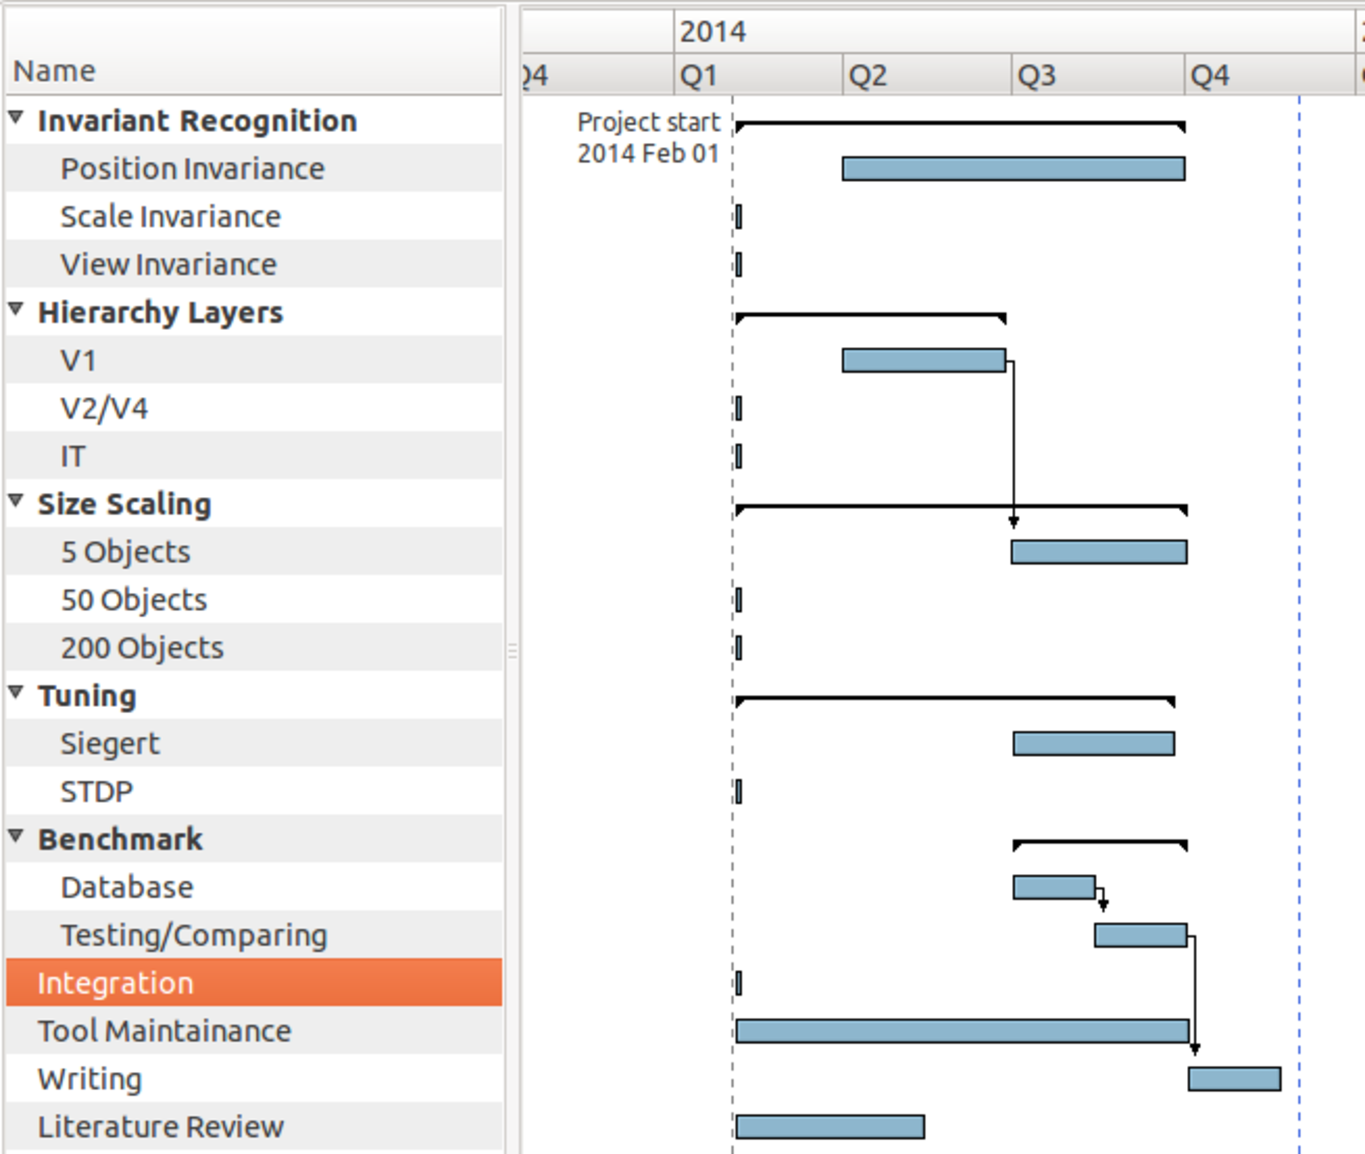
\includegraphics[width=0.8\textwidth]{pics/gantt.pdf}
	\caption{Gantt chart of the work flow for the first milestone.
	The main research works are listed on the left.
%	Different from the example, in the following work, not only achieving a milestone but also any increase in any dimension will result in tuning and benchmark testing.
	}
	\label{Fig:gantt}
\end{figure}
\subsection{Invariant Object Recognition}
As stated previously the brain recognises huge number of objects rapidly with ease even in noisy natural scenes. We will explore the invariant object recognition in three features: position, scale and viewing angle.
%While the major stumbling crux of the computer object recognition systems lies in the invariance problem.
%To explore the invariant object recognition of the brain in a biologically plausible way is the right place to solve the computational difficulty.
\subsubsection{Position Invariance}
Position invariance in the lower level of V1-liked neurons has been achieved in the preliminary work by convolving receptive fields with Gabor kernels.
The following work in accordance with Figure~\ref{Fig:3Dplan} will focus on expanding the position invariance to higher hierarchical levels of the ventral stream.
\subsubsection{Scale Invariance}
Similar to orientation detection, V1 provides overcomplete population re-representations of visual image on the features of scale, frequency and orientation.
It forms the basis of scale invariant object recognitions.
Likewise, integrating the features into the higher abstraction of layered network to recognise more complex figures will require a tense work on tuning.
\subsubsection{View Invariance}
A difficult specificity-invariance trade-off occurs in view invariant recognition tasks, since the recogniser should be able to discriminate different objects while at the same time also tolerating to viewing angle transformations.
Learning will play a very important role in this work, where objects observed with multiple view points can be recognised even if only single view point is presented during training.
\subsection{Modelling the Ventral Visual Pathway}
As the visual information propagates through the ventral stream (via visual area V1, V2/V4 and IT), neurons become selective for increasingly complex features. 
Along with this growing complexity of the preferred stimulus, neurons become more and more tolerant to the position and scale of the stimulus within their receptive fields.
Inspired from the functional behaviour of the biological data (many have been mentioned in Section~\ref{sec:bio}), this work will mimic the neural activity of each hierarchy layer by LIF neurons.
 
%To satisfy the functional discoveries, this work will employ learning and compare with biological data.
%This work will ask for a close collaboration with neuroscience to gather biological data for both training and testing.
\subsection{Size Scaling}
The milestones set for the dimension of number of classes/objects is in accordance with experimental data from the study of neuroscience.
In work by~\cite{hegde2004temporal}, the classical receptive field of the V2 cell consists of 48 grating stimuli and 80 contour stimuli; while Zoccolan et al.~\cite{zoccolan2007trade} tested and recorded the activity of the IT neurons of monkeys with 213 grayscale pictures of isolated real-world objects.

Thanks to the massively-parallel neural simulations possible in the SpiNNaker system, implementing real-time invariant object recognition becomes possible.
However, it also requires the supporting software development to support larger neural networks than currently possible.  
\subsection{Integration}
To reach the milestone of building an object recognition system with position, scale and view invariance, integration of these separate models will be a challenge.
It not only requires placing the models physically together but also merging their functions.
As illustrated in Section~\ref{sec:orIT}, single neurons are tuned to different features and object identities.
This work requires further investigation into population coding and learning. 
\subsection{Tuning}
Tuning is the key to make the object recognition system a success.
In preliminary work, Siegert transformation functions are used to adjust perceptral weights for spiking LIF neurons.
This is a strong indicator of the feasibility of the work.
However, learning algorithms such as STDP in spiking neural networks are must be employed to make the system more biologically plausible.
It is hoped that, this work will provoke further study of learning algorithms on SpiNNaker.
\subsection{Benchmarking Performance}
The performance of the real-time recognition system will be evaluated of each milestone to validate the success of the models.
The neural activities and recognition rate will be compared with biological data which will act as a benchmark.
\subsubsection{Building a Dataset}
Building a well-labelled retinal output dataset is essential in spike-based object recognition study.
Unified benchmarks with AER format will be ideal for SNN study, because of its non-frame, event-based fashion.
These benchmark datasets will also make it possible for other researchers to test their SNN model without a silicon retina present.
It is hoped that this would boost communication, comparison and collaboration within the community.
This work also requires lively discussion and cooperation with neuroscientists, where data can be derived and tested.
\subsubsection{Testing/Comparing}
The testing and comparing on the dataset will verify the reliability of the models.
The neural responses of single or populated neurons to the same dataset will be analysed in firing rate and response time.
By comparing with the biological data, the model can be rectified and improved.
The more data it compares with, the closer it could untangle the object representation. 


%\subsection{Optional: Action Recognition}
%vision attention.
%short-term memory.
%\subsection{Optional: Sensor Fusion with Auditory Processing}
%platform.
%applications as lip-reading and speaker identification.

